\documentclass[11pt,reqno]{article}
\usepackage{amsmath,amssymb,mathrsfs,amsthm}
\usepackage[UTF8]{ctex}
%\usepackage{xeCJK}
%\setCJKmainfont{SimSum}

\usepackage{graphicx,cite,cases}
%\usepackage[pagewise]{lineno}\linenumbers
%\usepackage{refcheck}
\usepackage{xcolor}
\usepackage{bm}			% 公式加粗
\usepackage{tabularx}   % 绘制定宽表格
\usepackage{authblk}	% 添加更多作者信息
\usepackage{appendix} 	% 生成附录
\usepackage{listings}   % 附录里的代码, 支持语言高亮
\usepackage{hyperref}   % 超链接, 自动跳转
\usepackage{subfigure}  % 插入多张图片
\hypersetup{hypertex=true,	% 定义超链接效果
colorlinks=true,
linkcolor=blue,
anchorcolor=blue,
citecolor=blue}

\setlength{\topmargin}{-1.5cm}
\setlength{\oddsidemargin}{0.0cm}
\setlength{\evensidemargin}{0.0cm}
\setlength{\textwidth}{16.7cm}
\setlength{\textheight}{23cm}
\headheight 20pt
\headsep    26pt
\footskip 0.4in

%%%%% 关于公式编号问题 %%%%%
%统一用equation环境
%如果需要加括号用\begin{cases}
%如果公式过长需要分行用\begin{split}
%如果一个equation里面需要多个公式, emmm没研究过

\newtheorem{theorem}{Theorem}[section]
\newtheorem{corollary}[theorem]{Corollary}
\newtheorem{lemma}[theorem]{Lemma}
\newtheorem{proposition}[theorem]{Proposition}
\newtheorem{remark}[theorem]{Remark}
\newtheorem{definition}[theorem]{Definition}
\numberwithin{equation}{section}


\renewcommand{\d}{\,\mathrm d}
\usepackage{algorithm,algorithmicx}  %写伪代码
\usepackage{algpseudocode}			% 写伪代码
%%%%%% 算法部分改为中文显示 %%%%%%%%%
%%\floatname{algorithm}{算法}
\renewcommand{\algorithmicrequire}{\textbf{Input:}}
\renewcommand{\algorithmicensure}{\textbf{Output:}}

%% Ctrl+Alt+R 编译
%% Ctrl+Alt+V 打开文档

\begin{document}

\title{微分方程数值解计算实习Lecture 4}

\author{朱荃凡}
\affil{(吉林大学数学系计算唐班)}
\date{\today}

\maketitle

\vspace{50pt}

\section{问题重述}
用二次元在均匀网格下求解边值问题\eqref{Eqn11}的数值解:
\begin{equation}\label{Eqn11}
	\begin{split}
	&-y''+\dfrac{\pi^2}{4}y=\dfrac{\pi^2}{2}\sin\dfrac{\pi}{2}x,\ 0<x<1,\\
	&\ \ y(0)=0,\qquad y'(1)=0.
	\end{split}
\end{equation}
要求:
\begin{itemize}
	\item  画出数值解的图像
	\item 对$[0,1]$区间均匀剖分成$N=10,20,30,\cdots,200$份,计算数值解和真解
	 \[u*=\sin\dfrac{\pi}{2}x\]
	的$L^2$误差和$H^1$误差,计算其关于网格长度$h=1/N$的数值收敛阶.
	\item 计算系数矩阵的条件数, 并用loglog()函数作图表示.
\end{itemize}

\newpage

\section{算法设计}

二次有限元和线性有限元除了基函数选区的不同以外,其余部分基本没有变化.所以我们主要
来看基函数带来的变化.



\subsection{生成刚度矩阵stiffnessMatrix()}

因为有限元次数的增加,刚度矩阵的大小变成了$2N+1\times2N+1$,但是剖分数仍然是不变的.
我们仍然逐区间的考虑问题,在区间$[0,h]$上,基函数可以被表达为
\begin{equation}
	\left\{\begin{matrix}
		\varphi_r(x)=2(\frac xh-\frac{1}{2})(\frac xh-1),&0\le x\le h, \\
		 \varphi_m(x)=4(\frac{x}{h})(1-\frac{x}{h} ),\quad\ \  & 0\le x\le h,\\
		\varphi_l(x)=2(\frac{x}{n} )(\frac xh-\frac{1}{2}),\quad\ \ &0\le x\le h.
		\end{matrix}\right.
\end{equation}
想要得到其他区间上的基函数平移即可.而事实上我们连平移都不需要,因为我们使用基函数是为了
得到高斯积分结点处的函数值.而基函数在每个小区间上的形状相同,高斯积分节点也对应相同.
于是我们可以直接保存基函数和其导数在$[0,h]$上高斯积分结点处的函数值,在使用到的时候
调用即可.不过需要注意,这种方法仅适用于等距剖分.

\begin{figure}[h]
	\centering
	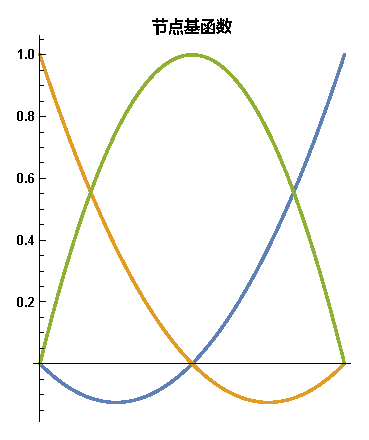
\includegraphics[width=0.4\textwidth]{Basisfunction.eps}

\end{figure}

有了节点基函数的表达公式,单元刚度矩阵可以被求解出来.由于使用了二次元,单元刚度矩阵
的大小是$3\times3$的.这里既可以手动求解, 也可以使用高斯积分公式.最终就得到了整体的
刚度矩阵.

\subsection{其余求解部分}

算法的其他部分效仿线性元的求解过程,并无较大改动.但是有一点值得注意,画真解和数值解误差图像时,
其横坐标是"自由度"而不是剖分数或者节点数量,换句话说在二次元中对应的横坐标为$2N-1$
(总共有$N+1$个节点和$N$个半节点,减去两个边值条件).


\section{程序结果}
\subsection{数值解图像}
这里展示了剖分数$N=10$和$N=50$时的图像,其中橙色圆点表示数值解,黑色实线表示真解. 
\\[-20pt]
\begin{figure}[h]
	\centering
	  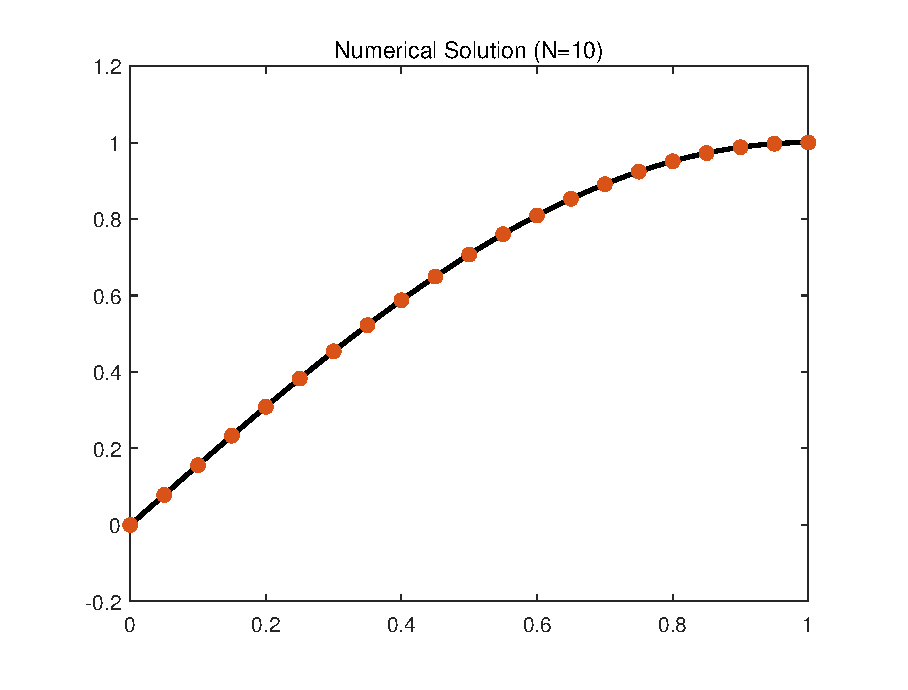
\includegraphics[width=0.6\textwidth]{N=10.eps}
	  \caption{真解和数值解}
\end{figure}

\subsection{误差和收敛阶}
接下来计算画出和收敛阶, 从图二图三中可以看出$H1$误差的收敛速度是$o(h^2)$,\ 
$L2$误差的收敛速度是$o(h^3)$,这比线性远快了一阶.因此对于一次元需要一千个剖分才能达到的精度,
对于二次元100个剖分就可以达到,这进而极大的减少了计算量。
\begin{figure}[h]
	\centering
	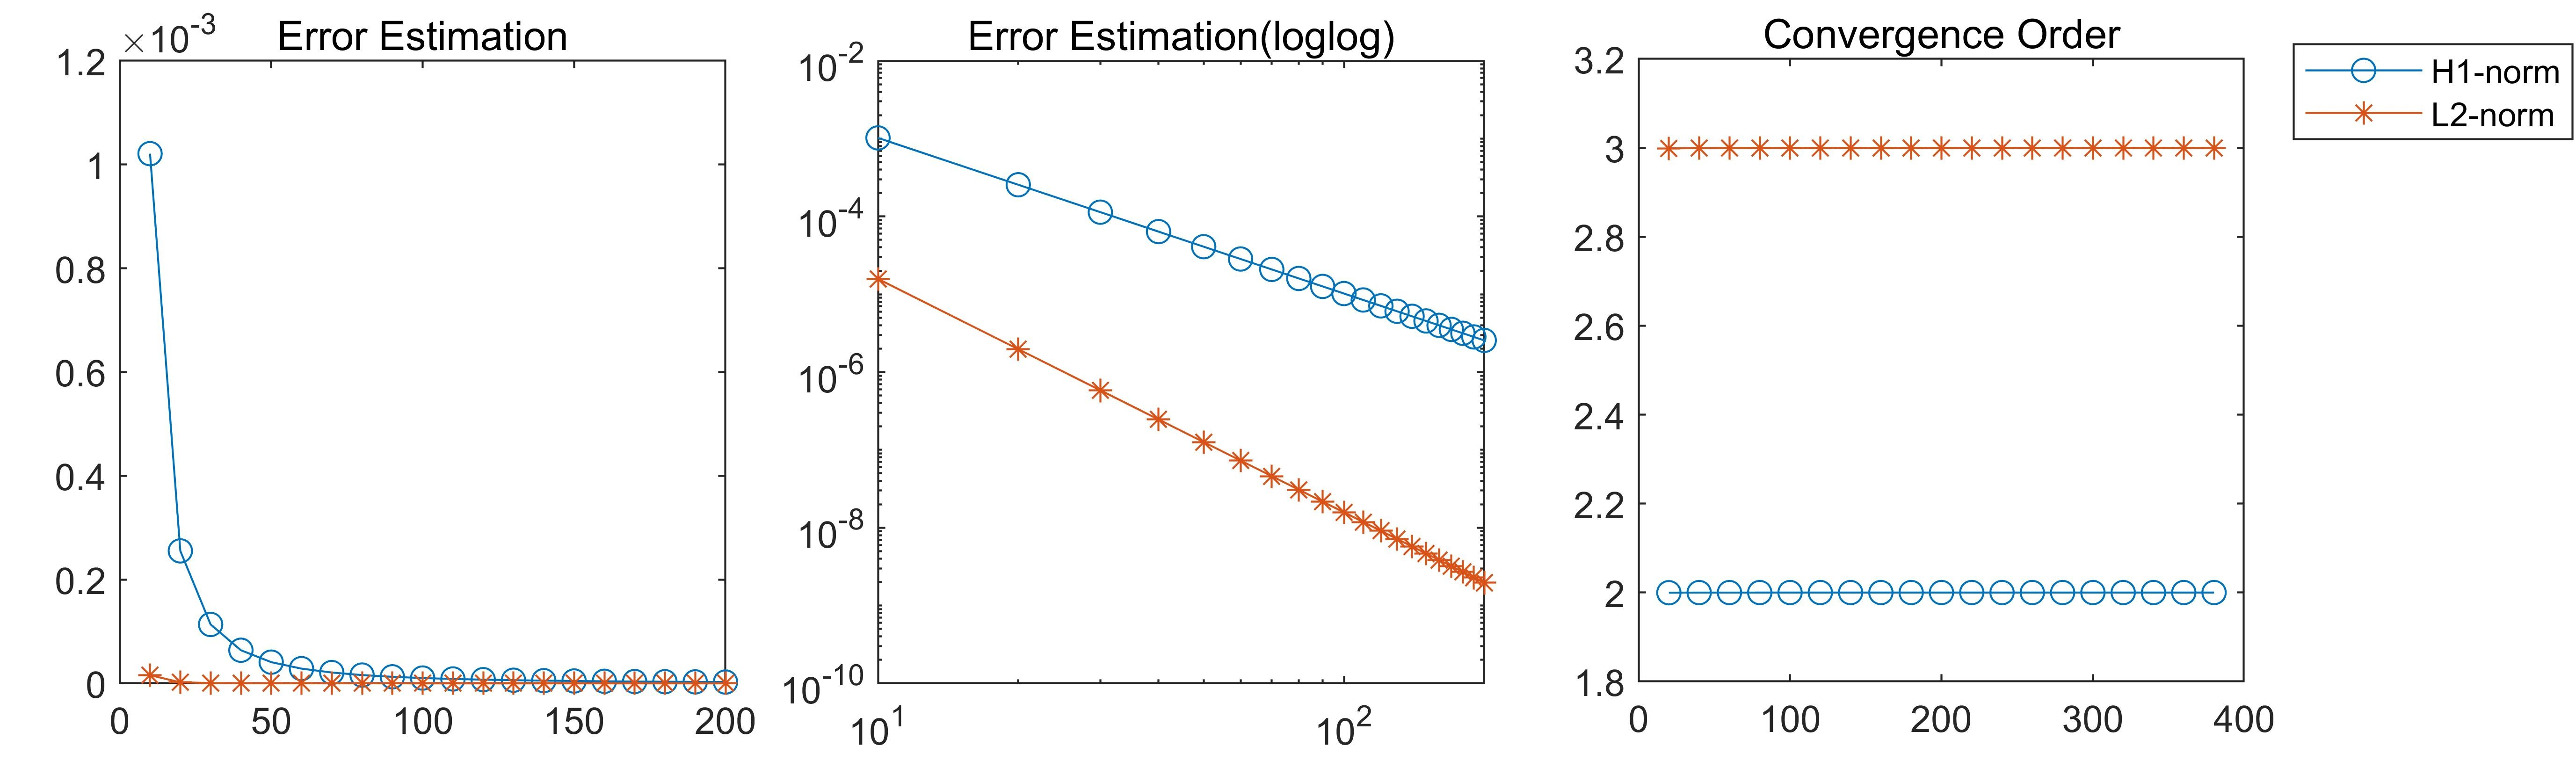
\includegraphics[width=\textwidth]{Error.jpg}
	\caption{误差和收敛阶}
\end{figure}

\newpage

\subsection{矩阵条件数}
最后是刚度矩阵的条件数. 我们画出如下的图像,其中图一是矩阵条件数与矩阵维数的双对数图,图二是发散阶.
其发散阶仍然是二阶的,但是平方项的系数对比线性元会稍大一些.
\begin{figure}[h]
	\centering
	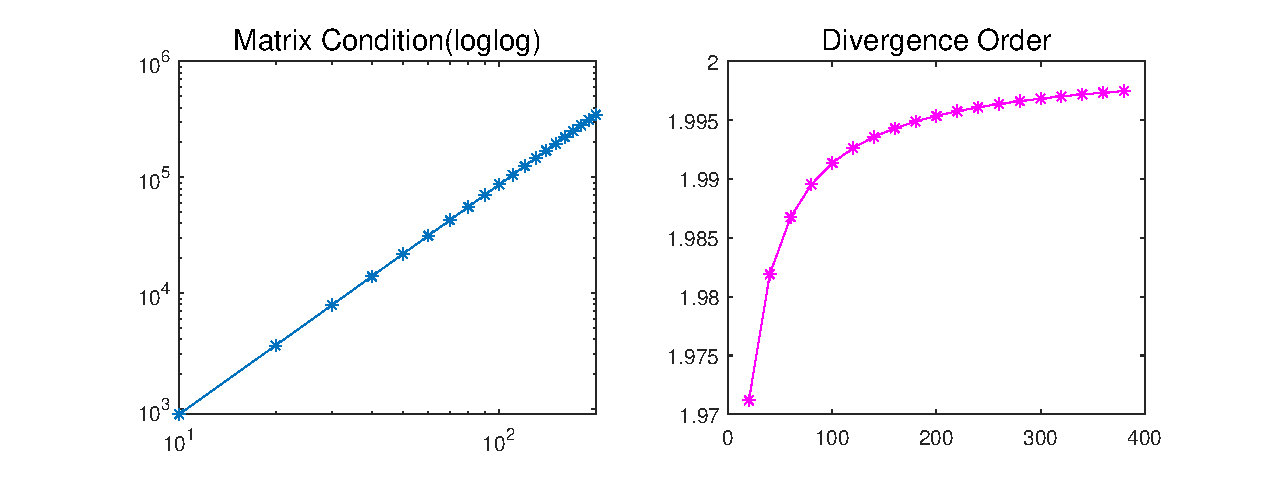
\includegraphics[width=\textwidth]{Condition.eps}
	\caption{系数矩阵条件数}
\end{figure}



\end{document}
